\documentclass[addpoints]{exam}
\usepackage[utf8]{inputenc}
\usepackage[portuguese]{babel}
\usepackage[LGRgreek]{mathastext}
\usepackage{graphicx,graphics}
\usepackage{hyperref}
%\usepackage{framed}
\usepackage{multirow}
\usepackage{booktabs}

%%% INÍCIO DOS COMANDOS ACRESCENTADOS NO NETBOOK %%%%%%%%%%%%%%%%%%%
\newcommand*{\renameenviron}[1]{%
  \expandafter\let\csname exam-#1\expandafter\endcsname
      \csname #1\endcsname
  \expandafter\let\csname endexam-#1\expandafter\endcsname
      \csname end#1\endcsname
  \expandafter\let\csname #1\endcsname\relax
  \expandafter\let\csname end#1\endcsname\relax
}
\renameenviron{framed}
\renameenviron{shaded}
\renameenviron{leftbar}
%%% FIM DOS COMANDOS ACRESCENTADOS NO NETBOOK %%%%%%%%%%%%%%%%%%%
\usepackage{framed}

\footer{}{\thepage}{}

\renewcommand{\arraystretch}{1.3}
%\setlength{\tabcolsep}{pt}
 
\pointpoints{ponto}{pontos}
\bonuspointpoints{ponto extra}{pontos extra}
 
\totalformat{Pregunta \thequestion: \totalpoints pontos}
 
\chqword{Pregunta}
\chpgword{Página}
\chpword{Pontos}
\chbpword{Pontos extra}
\chsword{Pontos obtidos}
\chtword{Total}

\hqword{Questão}
\hpgword{Página}
\hpword{Pontos}
\hsword{Pontos obtidos}
\htword{Total}

 
\begin{document}
 
\large

\begin{center}
\Large
\textbf{Laboratório de Eletrônica Básica II – EE641}
\end{center}

\large
\vspace{2mm}

\noindent\textbf{Profs.:} Dr. Eduardo T. Costa \hfill \textbf{Turma 01/2022} \\
\textbf{PED:} Mathias Scroccaro Costa \hfill %\textbf{e-mail:} mathias.scroccaro@gmail.com

\normalsize
 
\vspace{5mm}
 

 
\noindent\makebox[0.72\textwidth]{Nome: \enspace\hrulefill}
\hfill
\makebox[0.2\textwidth]{RA: \enspace\hrulefill}

\vspace{5mm}

\noindent\makebox[0.72\textwidth]{Nome: \enspace\hrulefill}
\hfill
\makebox[0.2\textwidth]{RA: \enspace\hrulefill}

\vspace{5mm}

\noindent\makebox[0.72\textwidth]{Nome: \enspace\hrulefill}
\hfill
\makebox[0.2\textwidth]{RA: \enspace\hrulefill}


%\begin{center}
%\gradetable[h][questions]
%\end{center}

\vspace{2mm}


\begin{center}
\large
\textbf{CONVERSOR DIGITAL PARA ANALÓGICO}
\normalsize
\end{center}

\begin{questions}

\section*{Conversor Digital para Analógico}

\question Monte o circuito Conversor Digital para Analógico (DAC) em \textbf{placa furada padrão}, conforme o esquemático da Figura \ref{cir:1}. Conside ``C'' com valor de 1 uF.

\begin{parts} 

\part Com auxílio de um gerador de sinais, insira uma forma de onda quadrada com amplitude de 1 V, frequência de 10 Hz e \textit{offset} de 0,5 V (desta maneira, tensão mínima 0 V e máxima 1 V) nas entradas D0 a D7 do circuito. Monitore com um osciloscópio a tensão de pico na saída do circuito, no borne ``Teste DAC ''. Complete a Tabela \ref{tab:1}.
%\begin{subparts}
%\subpart Desenvolva o algoritmo e grave no microcontrolador Arduino;
%\subpart \textbf{Desplugue} a interface USB do microcontrolador;
%\subpart Reconfira se a tensão entre os nós +9 V e GND do circuito montado é $\geq$ 7 V e também $\leq$ 12 V;
%\subpart Conecte o GND do circuito montado ao GND do Arduino;
%\subpart Conecte o nó +9 V à entrada Vin do Arduino (\textbf{ATENÇÃO}, não é a entrada 5 V!);
%\subpart Conecte D0 a D7 as GPIOs do Arduino;
%\end{subparts}

\begin{figure}[h!]
\begin{center}
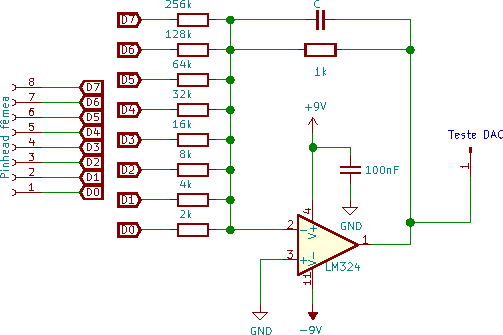
\includegraphics[width=0.8\textwidth]{imagens/dac1.pdf}
\end{center}
\caption{Circuito conversor digital para analógico.}
\label{cir:1}
\end{figure}

\begin{table}[h!]
\centering
\begin{tabular}{|c|c|c|c|c|c|c|c|c|c|}
\hline
D0 & D1 & D2 & D3 & D4 & D5 & D6 & D7 & \begin{tabular}[c]{@{}c@{}}Teste DAC [Vp]\\ (calculado)\end{tabular} & \begin{tabular}[c]{@{}c@{}}Teste DAC [Vp]\\ (osciloscópio)\end{tabular} \\ \hline
1 & 0 & 0 & 0 & 0 & 0 & 0 & 0 &  &  \\ \hline
0 & 1 & 0 & 0 & 0 & 0 & 0 & 0 &  &  \\ \hline
0 & 0 & 1 & 0 & 0 & 0 & 0 & 0 &  &  \\ \hline
0 & 0 & 0 & 1 & 0 & 0 & 0 & 0 &  &  \\ \hline
0 & 0 & 0 & 0 & 1 & 0 & 0 & 0 &  &  \\ \hline
0 & 0 & 0 & 0 & 0 & 1 & 0 & 0 &  &  \\ \hline
0 & 0 & 0 & 0 & 0 & 0 & 1 & 0 &  &  \\ \hline
0 & 0 & 0 & 0 & 0 & 0 & 0 & 1 &  &  \\ \hline
1 & 1 & 1 & 1 & 1 & 1 & 1 & 1 &  &  \\ \hline
\end{tabular}
\caption{Dados do medidos do conversor Digital para Analógico}
\label{tab:1}
\end{table}

\pagebreak

\part (PÓS EXPERIMENTO) Explique o funcionamento do conversor digital para analógico montado. Qual topologia o amplificador operacional está disposto no circuito?
\begin{framed}
\vspace{7cm}
\end{framed}

\pagebreak

\part (PÓS EXPERIMENTO) Encontre a função de transferência algébrica do circuito, ou seja, Vout(D0, D1,D2,D3,D4,D4,D5,D6,D7). Considere níveis de tensão analógicos para as entradas D0 a D7. Desconsidere o efeito da capacitância C. 
\begin{framed}
\vspace{12cm}
\end{framed}

\part (PÓS EXPERIMENTO) A capacitância C contribui ao caráter filtro no circuito. Qual é o tipo e a frequência de corte do filtro em questão? 
\begin{framed}
\vspace{6cm}
\end{framed}

\end{parts}

\end{questions}

\end{document}
